\chapter{The Foundations of Restorative Gravity}
\label{chap:restorative_gravity}

\begin{quote}
    \centering
    \textit{``Tensio Condensatur, Spatiotemporis Emergit, Gravitas Integrata''}
\end{quote}

\vspace{0.5em}
\noindent Standard General Relativity describes gravity as the geometric curvature of an empty, continuous spacetime manifold, offering no physical medium to explain how mass warps nothingness. Tension Field Theory (TFT) resolves this by moving beyond abstract geometry. Instead, we define gravity as a strict mechanical phenomenon: it is the restorative bulk tension of a highly elastic, discrete lattice actively attempting to crush a structural phase defect and return to absolute equilibrium.

\section{The First Law: Manifestation of Gravity (Restorative Tension)}
Gravity is the restorative tension of the Spacetime Lattice acting to suppress energetic vibration.

\begin{itemize}
    \item \textbf{Definition:} It is the mechanical response of the vacuum substrate attempting to minimize localized geometric strain—whether from permanent topological defects (invariant mass) or propagating transverse waves (effective mass)—to return to the flat equilibrium state of the Hard Floor.
    \item \textbf{Mechanism:} It manifests as a radial tension gradient, pulling inertial mass from regions of high static potential (unperturbed vacuum) toward regions of lower potential (matter-induced sinks).
\end{itemize}

\section{The Gravitational Constant ($G$): The Scale-Invariant Coupling Efficiency}
In \hyperref[part:one]{Part I} (\hyperref[app:fractal_architecture]{Appendix \ref*{app:fractal_architecture}}), we demonstrated mathematically that the Gravitational Constant ($G$) is not merely a fundamental number, but the scale-invariant coupling efficiency of the vacuum architecture. It represents the structural cost incurred when projecting tension from the rigid Substrate (Hard Floor) into the flexible layers of the continuum.

While its observable value is mediated by the specific geometry of the Soft Floor node ($J_{\mathrm{D}}$), the architecture ensures that this fundamental efficiency is conserved across all scales. We define $G_i$ as the ratio of the Substrate's source area ($A_{\mathrm{S}}$) to the Structural Mass Moment of the target layer ($J_i$), modulated by the lattice energy potential ($c_{\mathrm{E}}^2$):
\begin{equation}
    G_i = \mathcal{F}_i \cdot \left( \frac{c_{\mathrm{E}}^2 A_{\mathrm{S}}}{J_i} \right) \approx 6.67 \times 10^{-11} \text{ m}^3/(\text{kg}\cdot\text{s}^2)
\end{equation}

\textit{(See \hyperref[app:fractal_architecture]{Appendix \ref*{app:fractal_architecture}} for the fractal validation of $G$ across all scales, including the Nucleon).}

\begin{figure}[H]
    \centering
    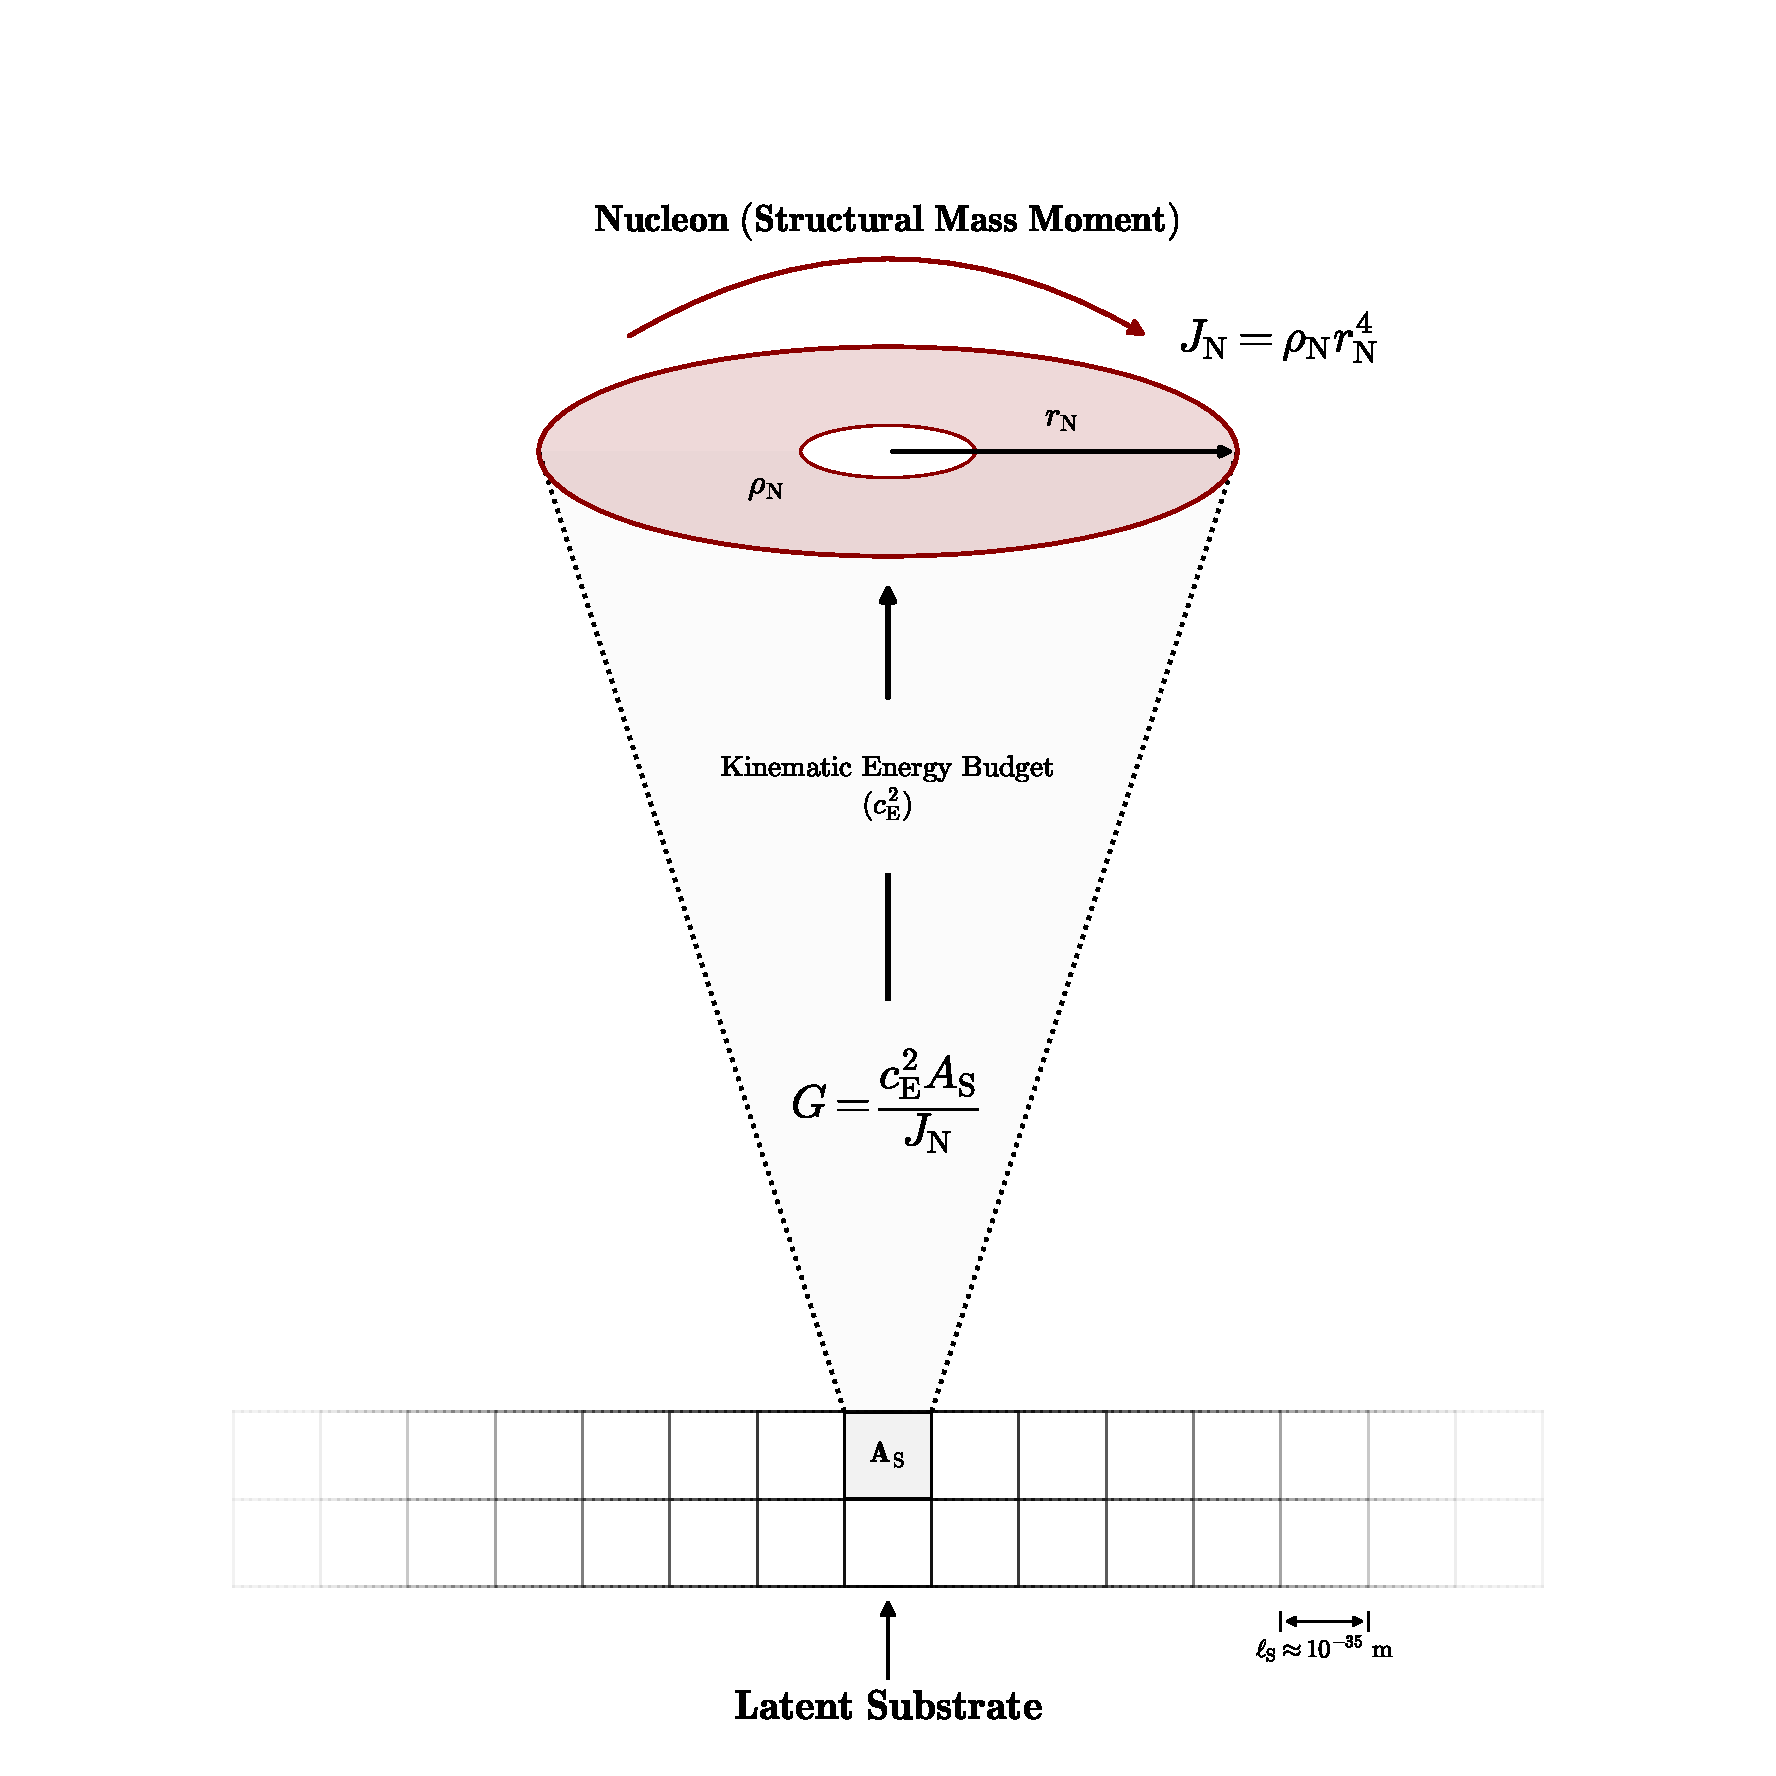
\includegraphics[width=0.9\textwidth]{Fig09_PartII_GravitationalConstantG.pdf}
    \caption{\textbf{The Mechanical Emergence of the Gravitational Constant ($G$).} This schematic illustrates the vertical architecture of gravity as a direct geometric coupling between the Latent Substrate (bottom) and the rotational inertia of the nucleon (top). The Gravitational Constant ($G$) functions as the scale-invariant coupling efficiency of this projection, mechanically defined by the ratio of the Substrate's absolute area ($A_{\mathrm{S}}$) to the Nucleon's Structural Mass Moment ($J_{\mathrm{N}}$), modulated by the kinematic energy budget ($c_{\mathrm{E}}^2$). For the nucleon, this rotation is governed by its mechanical radius ($r_{\mathrm{N}} \approx 0.88$ fm) and volumetric density ($\rho_{\mathrm{N}} \approx 5.86 \times 10^{17}$ kg/m$^3$).}
    \label{fig:gravitational_constant}
\end{figure}

\section{Gravitational Acceleration from the Tension Gradient ($-\nabla\tau$)}
Applying the derived gravitational constant, we find the gravitational tension ($\tau_{\mathrm{M}}$) for any spherical mass $M$ with radius $R$ in a vacuum:
\begin{equation}
    \tau_{\mathrm{M}} = \frac{G \cdot M \cdot \mu_{\mathrm{D}}}{R} \quad (\text{N/m})
\end{equation}

When this mass moves through the vacuum, it works against the lattice surface inertia ($\mu_{\mathrm{D}}$). Therefore, we define the gravitational acceleration ($g$) as the gradient of this tension potential normalized by the inertial density:
\begin{equation}
    g = - \left(\frac{1}{\mu_{\mathrm{D}}}\right) \frac{\mathrm{d}\tau_{\mathrm{M}}}{\mathrm{d}R} = -\frac{G \cdot M}{R^2}
\end{equation}

\section{The Equivalence Principle: Topological Cancellation}
Standard physics accepts the Equivalence Principle ($m_{\mathrm{inertial}} \equiv m_{\mathrm{gravitational}}$) as an empirical fact. TFT derives it as a strict topological necessity. In TFT, motion is not the continuous sliding of an object through empty space; it is a Discrete Structural Reconfiguration of the lattice.

\subsection*{The Mechanism of Inertia (Tying and Untying)}
\begin{itemize}
    \item \textbf{The Step (Reconfiguration):} To move, a particle must physically ``untie'' its 3D topological phase-knot from FCC lattice node A and simultaneously ``retie'' it onto the adjacent FCC lattice node B. It translates its phase state across their shared 2D interface ($\mu_{\mathrm{D}}$) via the phase gradient ($-\nabla\phi$).
    \item \textbf{The Drive (Gravity):} The vacuum substrate naturally seeks a flat equilibrium. It actively pulls on the topological knot to close the structural tension deficit.
    \item \textbf{The Cost (Inertia):} The knot resists this reconfiguration. The more complex the phase topology (higher density), the more ``hydrodynamic impedance'' the field exerts against the change.
\end{itemize}

\subsection*{Why All Masses Fall at the Same Rate}
Consider two objects: a dense Lead Ball (complex knot) and a Wood Ball (simple knot).

\vspace{0.3em}
\noindent\textbf{1. The Lead Ball (High Density Topology):}
\begin{itemize}
    \item \textit{Gravity (The Drive):} Creates a massive tension deficit far from equilibrium. The vacuum relaxation creates a massive pull.
    \item \textit{Inertia (The Resistance):} Has thousands of structural loops to ``untie and retie'' for every step. The hydrodynamic impedance is massive.
\end{itemize}

\vspace{0.3em}
\noindent\textbf{2. The Wood Ball (Low Density Topology):}
\begin{itemize}
    \item \textit{Gravity (The Drive):} Creates a small tension deficit. The vacuum pull is weak.
    \item \textit{Inertia (The Resistance):} Easy to untie and retie. The hydrodynamic impedance is weak.
\end{itemize}

\noindent\textbf{Conclusion:} The topology of the mass scales the pull (Gravity) and the resistance (Inertia) by the exact same geometric factor. Nature does not ``know'' to make them equal; mechanically, the structure being pulled is the exact same structure resisting the pull.
\begin{equation}
    a = \frac{F_{\mathrm{gravity}}}{m_{\mathrm{inertia}}} = \text{Constant } (g)
\end{equation}

\section{Bound-Orbit Strain Coupling and Perihelion Precession}
\label{sec:perihelion_strain_coupling}

The equivalence-principle derivation above establishes why all localized mass defects experience the same radial acceleration in the Newtonian limit. However, a bound orbit is not merely radial free fall. A planet is a three-dimensional topological defect aggregate moving tangentially through the radial strain field established by the central mass.

This produces a distinct conservative correction to the Newtonian bound-orbit acceleration. The correction is not a dark-matter impedance effect and not an optical propagation delay. It is a local bound-orbit strain effect caused by the coupling between the radial Soft Floor strain potential and the tangential transport of the orbiting mass defect.

For a central mass \(M\), the radial Soft Floor strain potential per unit mass is
\begin{equation}
    \Phi_\tau(r)
    =
    -
    \frac{GM}{r}.
\end{equation}

A bound orbiting mass moving with tangential speed \(v_\perp\) consumes a dimensionless fraction of the Soft Floor kinematic capacity,
\begin{equation}
    \frac{v_\perp^2}{c_{\mathrm{E}}^2}.
\end{equation}

Therefore, the leading conservative specific orbital strain-potential coupling is
\begin{equation}
    \Phi_{\mathrm{orb}}
    =
    \Phi_\tau
    \frac{v_\perp^2}{c_{\mathrm{E}}^2}.
\end{equation}

For the weak-field spherical bound-orbit problem, the specific orbital angular momentum is conserved:
\begin{equation}
    \ell_{\mathrm{orb}}
    =
    rv_\perp.
\end{equation}

After imposing this bound-orbit reduction, the orbital strain potential becomes
\begin{equation}
    \Phi_{\mathrm{orb}}^{(\mathrm{red})}
    =
    -
    \frac{GM\ell_{\mathrm{orb}}^2}
    {c_{\mathrm{E}}^2r^3}.
\end{equation}

This reduced potential is not a fully general velocity-dependent field potential for arbitrary motion. It is the reduced central-orbit strain potential obtained after applying angular-momentum conservation to a weak-field, spherical, conservative bound orbit.

The radial derivative of this cubic reduced strain-potential term produces the additional inward bound-orbit correction
\begin{equation}
    g_{\mathrm{orb}}
    =
    3g_{\mathrm{b}}
    \frac{v_\perp^2}{c_{\mathrm{E}}^2},
\end{equation}
where
\begin{equation}
    g_{\mathrm{b}}
    =
    \frac{GM}{r^2}.
\end{equation}

Thus, the inward acceleration magnitude for a weak-field massive bound orbit becomes
\begin{equation}
    g_{\mathrm{bound}}
    =
    g_{\mathrm{b}}
    +
    g_{\mathrm{orb}}
    =
    \frac{GM}{r^2}
    +
    \frac{3GM\ell_{\mathrm{orb}}^2}
    {c_{\mathrm{E}}^2r^4}.
\end{equation}

This correction leads directly to the weak-field post-Newtonian orbital equation
\begin{equation}
    \frac{\mathrm{d}^2u}{\mathrm{d}\varphi^2}
    +
    u
    =
    \frac{GM}{\ell_{\mathrm{orb}}^2}
    +
    \frac{3GM}{c_{\mathrm{E}}^2}u^2,
\end{equation}
where \(u=1/r\). This is the same reduced orbital equation obtained in General Relativity for the weak-field perihelion correction.

Therefore, TFT recovers the standard perihelion advance
\begin{equation}
    \Delta\varphi
    =
    \frac{6\pi GM}
    {a(1-e^2)c_{\mathrm{E}}^2}.
\end{equation}

The complete mechanical derivation is provided in \hyperref[app:perihelion_orbital_strain]{Appendix~\ref*{app:perihelion_orbital_strain}}.

In TFT interpretation, the non-closing orbit is not caused fundamentally by spacetime curvature. It is the cumulative orbital phase advance generated by the conservative cubic reduced Soft Floor strain potential of a bound topological defect moving through a radially pre-stressed lattice.

\section{The Galactic Rotation Solution (Cosmic Impedance)}
Standard physics fails to predict the rotation speeds of galaxies (the Dark Matter Problem) because it assumes the vacuum offers zero resistance \cite{Milgrom_1983}. TFT corrects this by introducing the Cosmic Impedance ($a_{\mathrm{D}}$) of the active vacuum FCC lattice. It is not that galaxies contain invisible mass; rather, the outer stars feel the viscous grip of the vacuum itself.

\begin{itemize}
    \item \textbf{Mechanism:} In the deep galactic outskirts, the acceleration is so weak that the stars can no longer ``cut'' through the lattice elastically. Instead, they must push against the Interstitial Condensate of the FCC active vacuum.
    \item \textbf{Result:} This condensate creates a hydrodynamic floor for gravity, leading to the Total Acceleration Law:
\end{itemize}
\begin{equation}
    g_{\mathrm{obs}} = g_{\mathrm{b}} + \sqrt{a_{\mathrm{D}} \cdot g_{\mathrm{b}}}
\end{equation}

\begin{itemize}
    \item \textbf{Inner Galaxy ($g \gg a_{\mathrm{D}}$):} The star moves too fast for the condensate to couple. The vacuum response is purely elastic (Newtonian).
    \item \textbf{Outer Galaxy ($g \ll a_{\mathrm{D}}$):} The star ``swims'' through the viscous lattice. The impedance term $\sqrt{a_{\mathrm{D}} \cdot g_{\mathrm{b}}}$ dominates, naturally flattening the rotation curve.
\end{itemize}
\textit{(See \hyperref[app:cosmic_impedance]{Appendix \ref*{app:cosmic_impedance}} for the derivation of $a_{\mathrm{D}}$ from the vacuum's kinematic viscosity).}

\section{The Master Acceleration Equation}
\label{sec:master_acceleration_equation}

While the galactic rotation solution explains the large-scale ``dark matter'' effect using cosmic impedance ($a_{\mathrm{D}}$), real astrophysical systems are complex. Galaxies are flattened disks, not perfect spheres, and gravitational influence cannot extend to infinity without violating finite-energy coherence. In addition, precision solar-system orbits require a separate post-Newtonian bound-orbit correction.

To avoid conflating these physically distinct regimes, TFT separates the gravitational response into two levels:

\begin{enumerate}
    \item the \textbf{environmental acceleration field}, governed by baryonic restorative gravity, geometric projection, and large-scale coherence screening;
    \item the \textbf{precision bound-orbit correction}, which applies only to massive bodies moving tangentially through a radial strain field.
\end{enumerate}

The environmental weak-field acceleration law is therefore
\begin{equation}
    g_{\mathrm{obs}}(R) = \Pi(R) \left[ g_{\mathrm{b}}(R) + \Xi(R)\sqrt{a_{\mathrm{D}}\,g_{\mathrm{b}}(R)} \right].
\end{equation}

\noindent\textbf{Variables:}
\begin{itemize}
    \item $\Pi(R)$: The radial projection operator. It corrects for anisotropic tension losses in non-spherical geometries, such as galactic disks, and accounts for geometric focusing or dilution of the radial tension field (See \hyperref[app:radial_projection]{Appendix~\ref*{app:radial_projection}}).

    \item $g_{\mathrm{b}}(R)$: The standard baryonic restorative acceleration due to visible matter. In spherical symmetry this reduces to the ordinary Newtonian field,
    \begin{equation}
        g_{\mathrm{b}}(R) = \frac{GM}{R^2}.
    \end{equation}

    \item $\Xi(R)$: The coherence screening function. It ensures that the vacuum halo fades at the cosmic coherence limit, preserving finite total energy (See \hyperref[app:cosmic_impedance]{Appendix~\ref*{app:cosmic_impedance}}).

    \item $a_{\mathrm{D}}$: The Lattice Impedance Acceleration, representing the large-scale ``dark matter'' effect generated by the interstitial condensate response of the active vacuum.
\end{itemize}

\noindent\textbf{Precision Bound-Orbit Extension:}

The environmental field above describes the source-generated radial acceleration structure of the active Soft Floor. It does not by itself include the reduced orbital correction responsible for perihelion precession, because that correction depends on the tangential motion of a massive bound test body.

For a massive body in a weak-field spherical bound orbit, the environmental acceleration is supplemented by the conservative orbital strain correction
\begin{equation}
    g_{\mathrm{bound}}(R,v_\perp) = g_{\mathrm{obs}}(R) + g_{\mathrm{orb}}(R,v_\perp),
\end{equation}
where
\begin{equation}
    g_{\mathrm{orb}}(R,v_\perp) = 3g_{\mathrm{b}}(R) \frac{v_\perp^2}{c_{\mathrm{E}}^2}.
\end{equation}

This term is not a dark-matter impedance term and not part of the static source field. It is a reduced bound-orbit correction obtained after imposing conservation of specific orbital angular momentum,
\begin{equation}
    \ell_{\mathrm{orb}} = Rv_\perp.
\end{equation}

Equivalently, in the spherical central-field limit,
\begin{equation}
    g_{\mathrm{orb}}(R,\ell_{\mathrm{orb}}) = \frac{3GM\ell_{\mathrm{orb}}^2}{c_{\mathrm{E}}^2R^4}.
\end{equation}

This correction produces the weak-field perihelion orbital equation
\begin{equation}
    \frac{\mathrm{d}^2u}{\mathrm{d}\varphi^2} + u = \frac{GM}{\ell_{\mathrm{orb}}^2} + \frac{3GM}{c_{\mathrm{E}}^2}u^2,
\end{equation}
and therefore the standard perihelion advance
\begin{equation}
    \Delta\varphi = \frac{6\pi GM}{a(1-e^2)c_{\mathrm{E}}^2}.
\end{equation}

The complete mechanical derivation is provided in \hyperref[sec:perihelion_strain_coupling]{Section~\ref*{sec:perihelion_strain_coupling}} and \hyperref[app:perihelion_orbital_strain]{Appendix~\ref*{app:perihelion_orbital_strain}}.

\noindent\textbf{Mechanical Interpretation:}

The environmental acceleration equation contains two source-field channels:
\begin{equation}
    g_{\mathrm{obs}} = \text{baryonic restorative gravity} + \text{cosmic impedance response}.
\end{equation}

The first term,
\begin{equation}
    g_{\mathrm{b}},
\end{equation}
is the baseline radial restorative acceleration produced by the tension gradient of the active Soft Floor.

The second term,
\begin{equation}
    \Xi(R)\sqrt{a_{\mathrm{D}}g_{\mathrm{b}}(R)},
\end{equation}
is the large-scale inductive response of the interstitial condensate. This term produces the galactic rotation effect normally attributed to particulate dark matter.

The perihelion correction belongs to a different category. It is a trajectory-dependent correction for massive bound orbits:
\begin{equation}
    g_{\mathrm{orb}} = 3g_{\mathrm{b}} \frac{v_\perp^2}{c_{\mathrm{E}}^2}.
\end{equation}
It appears only when a bound topological defect moves tangentially through a radial strain field.

Thus, TFT separates gravitational phenomenology into three controlled regimes:
\begin{equation}
    \text{Newtonian restorative field} \quad + \quad \text{large-scale condensate impedance} \quad + \quad \text{bound-orbit strain correction}.
\end{equation}

The first two define the environmental acceleration field. The third defines the precision post-Newtonian correction for massive bound orbits.

\noindent\textbf{Universal Application:} This acceleration hierarchy recovers the relevant gravitational limits without conflating field dynamics and trajectory-dependent orbital dynamics:

\begin{itemize}
    \item \textbf{Solar System} ($\Pi \approx 1, \Xi \to 0$): The cosmic-impedance term vanishes, and the environmental field reduces to ordinary Newtonian gravity:
    \begin{equation}
        g_{\mathrm{obs}} \approx g_{\mathrm{b}}.
    \end{equation}
    For precision bound-orbit dynamics, the additional conservative orbital strain correction gives
    \begin{equation}
        g_{\mathrm{bound}} \approx g_{\mathrm{b}} + g_{\mathrm{orb}}.
    \end{equation}
    The dominant term $g_{\mathrm{b}}$ recovers the Newtonian limit, while $g_{\mathrm{orb}}$ produces the observed weak-field perihelion precession.

    \item \textbf{Galactic Disk} ($\Pi \lesssim 1, \Xi \to 1$): The bound-orbit strain correction is negligible compared with the condensate impedance response. The environmental acceleration law reduces approximately to
    \begin{equation}
        g_{\mathrm{obs}} \approx \Pi(R) \left[ g_{\mathrm{b}}(R) + \sqrt{a_{\mathrm{D}}g_{\mathrm{b}}(R)} \right],
    \end{equation}
    recovering flat rotation curves consistent with the Tully--Fisher relation \cite{Tully_1977}.

    \item \textbf{Deep Cosmos} ($\Xi \to 0$): The coherence screening function suppresses the interstitial-condensate halo at large radius. The acceleration law returns to the finite-energy baryonic field,
    \begin{equation}
        g_{\mathrm{obs}} \approx \Pi(R)g_{\mathrm{b}}(R),
    \end{equation}
    recovering Keplerian decay and preventing the vacuum impedance halo from extending to infinite energy.

    \item \textbf{Black Hole Regime} ($\Pi > 1, \Xi \to 0$): The coherence-screened impedance term vanishes, while geometric focusing of the radial tension field amplifies the local gravitational response. In this regime, the active Soft Floor approaches the saturation condition $\alpha_{\mathrm{G}} \to 1$, leading to event-horizon formation as a mechanical phase transition rather than a geometric singularity.
\end{itemize}

This formulation keeps the master acceleration equation as an environmental field law while treating perihelion precession as the separate reduced bound-orbit correction required for post-Newtonian precision. It therefore avoids mixing a source-field acceleration with a trajectory-dependent orbital term.
